{插入排序的工作机理与很多人打牌时,整理手中牌时的做法差不多。每次摸牌后将它插入到左手一把牌中的正确位置。为了找到这张牌的正确位置,要将它和手中的每一张牌从右到左进行比较。}

{\textbf{算法描述:}每趟将一个待排序的关键字,按照其关键字值的大小顺序查找到适当位置,完成插入,直到待排序的关键字为空。代码如下:}

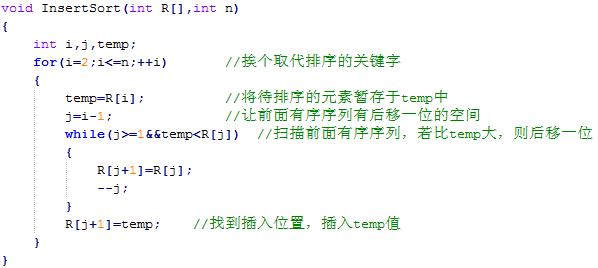
\includegraphics[width=3.70833in,height=1.66667in]{png-jpeg-pics/C128245F708560642ED13F460DF8388E.png}{}

{\textbf{算法分析:}直接插入排序的比较次数取决于原记录序列的有序程度。如果原始记录的关键字正好为递增顺序时,比较次数最少为n-1次;如果为递减顺序时,比较次数最多,为(n-1)(n+2)/2次,因此,直接插入排序的时间复杂度为O(n}\textsuperscript{2}{)。}
